\documentclass[10pt, handout]{beamer}
\usepackage{graphicx} % Required for inserting images
\usepackage{amsmath, amsthm, amssymb}
\usepackage{natbib}
\usepackage{xcolor}

% Theme and Color Configuration
% \usetheme{Madrid}
% \usecolortheme{beaver}
% \setbeamertemplate{frame footer}{\insertshortauthor}
% \setbeamertemplate{footline}{\insertshortauthor~(\insertshortinstitute)\hfill\insertshorttitle}

\setbeamerfont{title}{size=\large}
\setbeamerfont{author}{size=\small}
\setbeamerfont{date}{size=\scriptsize}
\setbeamerfont{normal text}{size=\small}
\setbeamerfont{frametitle}{size=\large}
\setbeamerfont{block title}{size=\normalsize}
\setbeamerfont{block body}{size=\small}
\setbeamerfont{author in head/foot}{size=\tiny}
\setbeamerfont{itemize/enumerate body}{size=\small}
\setbeamerfont{itemize/enumerate subbody}{parent=itemize/enumerate body, size=\footnotesize}
\setbeamerfont{itemize/enumerate subsubbody}{parent=itemize/enumerate body, size=\scriptsize}

\usefonttheme{serif}
% \usepackage[scaled=0.95]{newpxtext}
% \usepackage{newpxmath}
\usepackage[T1]{fontenc}
\usepackage{mathpazo}

\definecolor{darkred}{rgb}{0.55, 0.0, 0.0}
\definecolor{maroon(html/css)}{rgb}{0.5, 0.0, 0.0}
\setbeamercolor{title}{fg=darkred}
\setbeamercolor{frametitle}{fg=darkred}

\setbeamercolor{theorem title}{bg=maroon(html/css)!90!white, fg=white}
\setbeamercolor{theorem body}{bg=maroon(html/css)!20!white, fg=black}
\setbeamercolor{block title}{bg=maroon(html/css)!90!white, fg=white}
\setbeamercolor{block body}{bg=maroon(html/css)!20!white, fg=black}
\setbeamercolor{author in head/foot}{fg=black!30!white}
\setbeamercolor{title in head/foot}{fg=black!30!white}
\setbeamercolor{caption name}{fg=darkred}
\setbeamerfont{caption name}{size=\scriptsize}

\setbeamertemplate{itemize item}[ball]
\setbeamercolor{item}{fg=darkred}
\setbeamercolor{itemize subitem}{fg=darkred}
\setbeamercolor{enumerate item}{fg=darkred}
\setbeamercolor{navigation symbols}{fg=darkred, bg=darkred!20!white}
\setbeamertemplate{footline}{%
  \begin{beamercolorbox}[ht=2.5ex,dp=2.5ex,%
    leftskip=.3cm,rightskip=.3cm plus1fil]{title in head/foot}
    \leavevmode{\usebeamerfont{title in head/foot}%
      [\insertshorttitle, \insertframenumber]}
  \end{beamercolorbox}%
}
\setbeamertemplate{navigation symbols}{}

\setbeamertemplate{blocks}[rounded][shadow=true]



\title[AIPW\_NF]{Using Normalizing Flows for Weighting Estimators with Continuous Treatment}
\author[Park and Song]{Chanhyuk Park \quad Xiangyu Song}
\institute{Washington University in St. Louis}
\date{April 21, 2026}

\newcommand{\ind}{\perp\!\!\!\!\perp}
\DeclareMathOperator{\D}{D}

\begin{document}

\maketitle

%%% SLIDE 1: Motivation %%%
\begin{frame}
  \frametitle{Motivation}

  \begin{itemize}
    \item Causal inference under \textbf{unconfoundedness} relies on accurate propensity score estimation
    \item AIPW estimator is \textbf{doubly robust} and semiparametrically efficient
    \item \textbf{Continuous treatment} is common in political science:
    \begin{itemize}
      \item Amount of foreign aid on economic development
      \item Campaign spending on vote share
      \item Duration of peacekeeping missions on conflict recurrence
      \item Level of media exposure on political attitudes
    \end{itemize}
    \item Two challenges when treatment is continuous:
    \begin{itemize}
      \item Dichotomizing loses information on treatment effect heterogeneity
      \item No logit/probit analogue --- need to estimate a \textit{conditional density} $f(T \mid X)$
    \end{itemize}
    \item Existing approach: kernel density estimation (KDE)
    \begin{itemize}
      \item Sensitive to kernel choice and bandwidth
    \end{itemize}
    \item \textbf{Our proposal:} use \textit{Normalizing Flows} (NF) for propensity score estimation with continuous treatment
  \end{itemize}

\end{frame}

%%% SLIDE 2: AIPW with Continuous Treatment %%%
\begin{frame}
  \frametitle{AIPW with Continuous Treatment}
  
  \begin{itemize}
    \item Under unconfoundedness $T \ind Y(t) \mid X$ and overlap, the \textbf{dose--response function} is:
        \[
    m(t) = \mathbb{E}[Y(t)] = \mathbb{E}\!\left[\mu(t, X) + \frac{K_h(T - t)}{f(T \mid X)}\big(Y - \mu(T, X)\big)\right]
  \]
    
    \begin{itemize}
      \item $\mu(t, x) = \mathbb{E}[Y \mid T = t, X = x]$: outcome model
      \item $f(T \mid X)$: \textbf{generalized propensity score} (GPS)
      \item $K_h(\cdot)$: kernel with bandwidth $h$
    \end{itemize}

  \end{itemize}

  \vspace{0.3cm}
  \begin{block}{Double Robustness}
    Consistent if \textit{either} the outcome model $\mu$ or the GPS $f(T \mid X)$ is correctly specified \citep{robins1997curse}.
  \end{block}

\end{frame}

%%% SLIDE 3: Normalizing Flows %%%
\begin{frame}
  \frametitle{Normalizing Flows}
  
  \begin{itemize}
    \item \textbf{Idea:} transform a simple base distribution (e.g., Gaussian) into a complex target via invertible maps.
    \item \textbf{Change of variables:}
        \[
    p_{\mathbf{Y}}(\mathbf{y}) = p_{\mathbf{Z}}(\mathbf{f}(\mathbf{y})) \left| \det \D\mathbf{f}(\mathbf{y}) \right|
  \]
    \begin{itemize}
    \item $\mathbf{f}$: invertible transformation
    \item Exact density evaluation \& sampling
    \item No kernel/bandwidth choices needed
  \end{itemize}

  \end{itemize}

  
  \begin{figure}
    \centering
    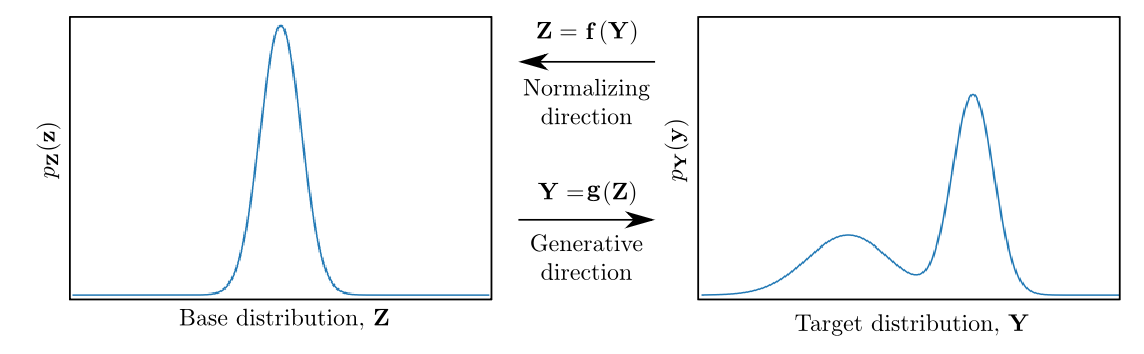
\includegraphics[width=0.8\linewidth]{../../figures/nf_graph.png}
    \caption{\scriptsize From \cite{kobyzev2021normalizing}}
  \end{figure}

\end{frame}

%%% SLIDE 4: Conditional NF for GPS %%%
\begin{frame}
  \frametitle{NF for Propensity Score Estimation}

  \begin{itemize}
    \item \textbf{Goal:} estimate the conditional density $f(T \mid X)$ using conditional NF
    \begin{itemize}
      \item Train a conditional NF: transformation parameters depend on covariates $X$
      \item Yields \textbf{exact} conditional density $\hat{f}(T \mid X)$ via change of variables
      \item Plug $\hat{f}(T \mid X)$ into the AIPW estimator as the GPS
    \end{itemize}
    \item \textbf{Advantages over KDE:}
    \begin{itemize}
      \item No kernel/bandwidth choices
      \item Captures complex, multimodal densities
      \item Scalable to higher-dimensional covariates
    \end{itemize}
  \end{itemize}

  \begin{figure}
    \centering
    \includegraphics[width=0.4\linewidth]{../../figures/cond_twomoons_truth.pdf}
    %\hfill
    \includegraphics[width=0.4\linewidth]{../../figures/cond_twomoons_resampled_model.pdf}
    \caption{\scriptsize Conditional two-moons: true density (left) vs.\ NF estimate (right)}
  \end{figure}

\end{frame}

%%% SLIDE 5: Simulation Results %%%
\begin{frame}
  \frametitle{Simulation Results}

  \begin{itemize}
    \item Compare DR estimators using: (1) true GPS, (2) residual KDE, (3) NF
    \begin{itemize}
      \item NF-based DR estimator performs \textbf{comparably to true GPS}
      \item Bias and RMSE decrease with $n$
    \end{itemize}
  \end{itemize}

  \begin{figure}
    \centering
    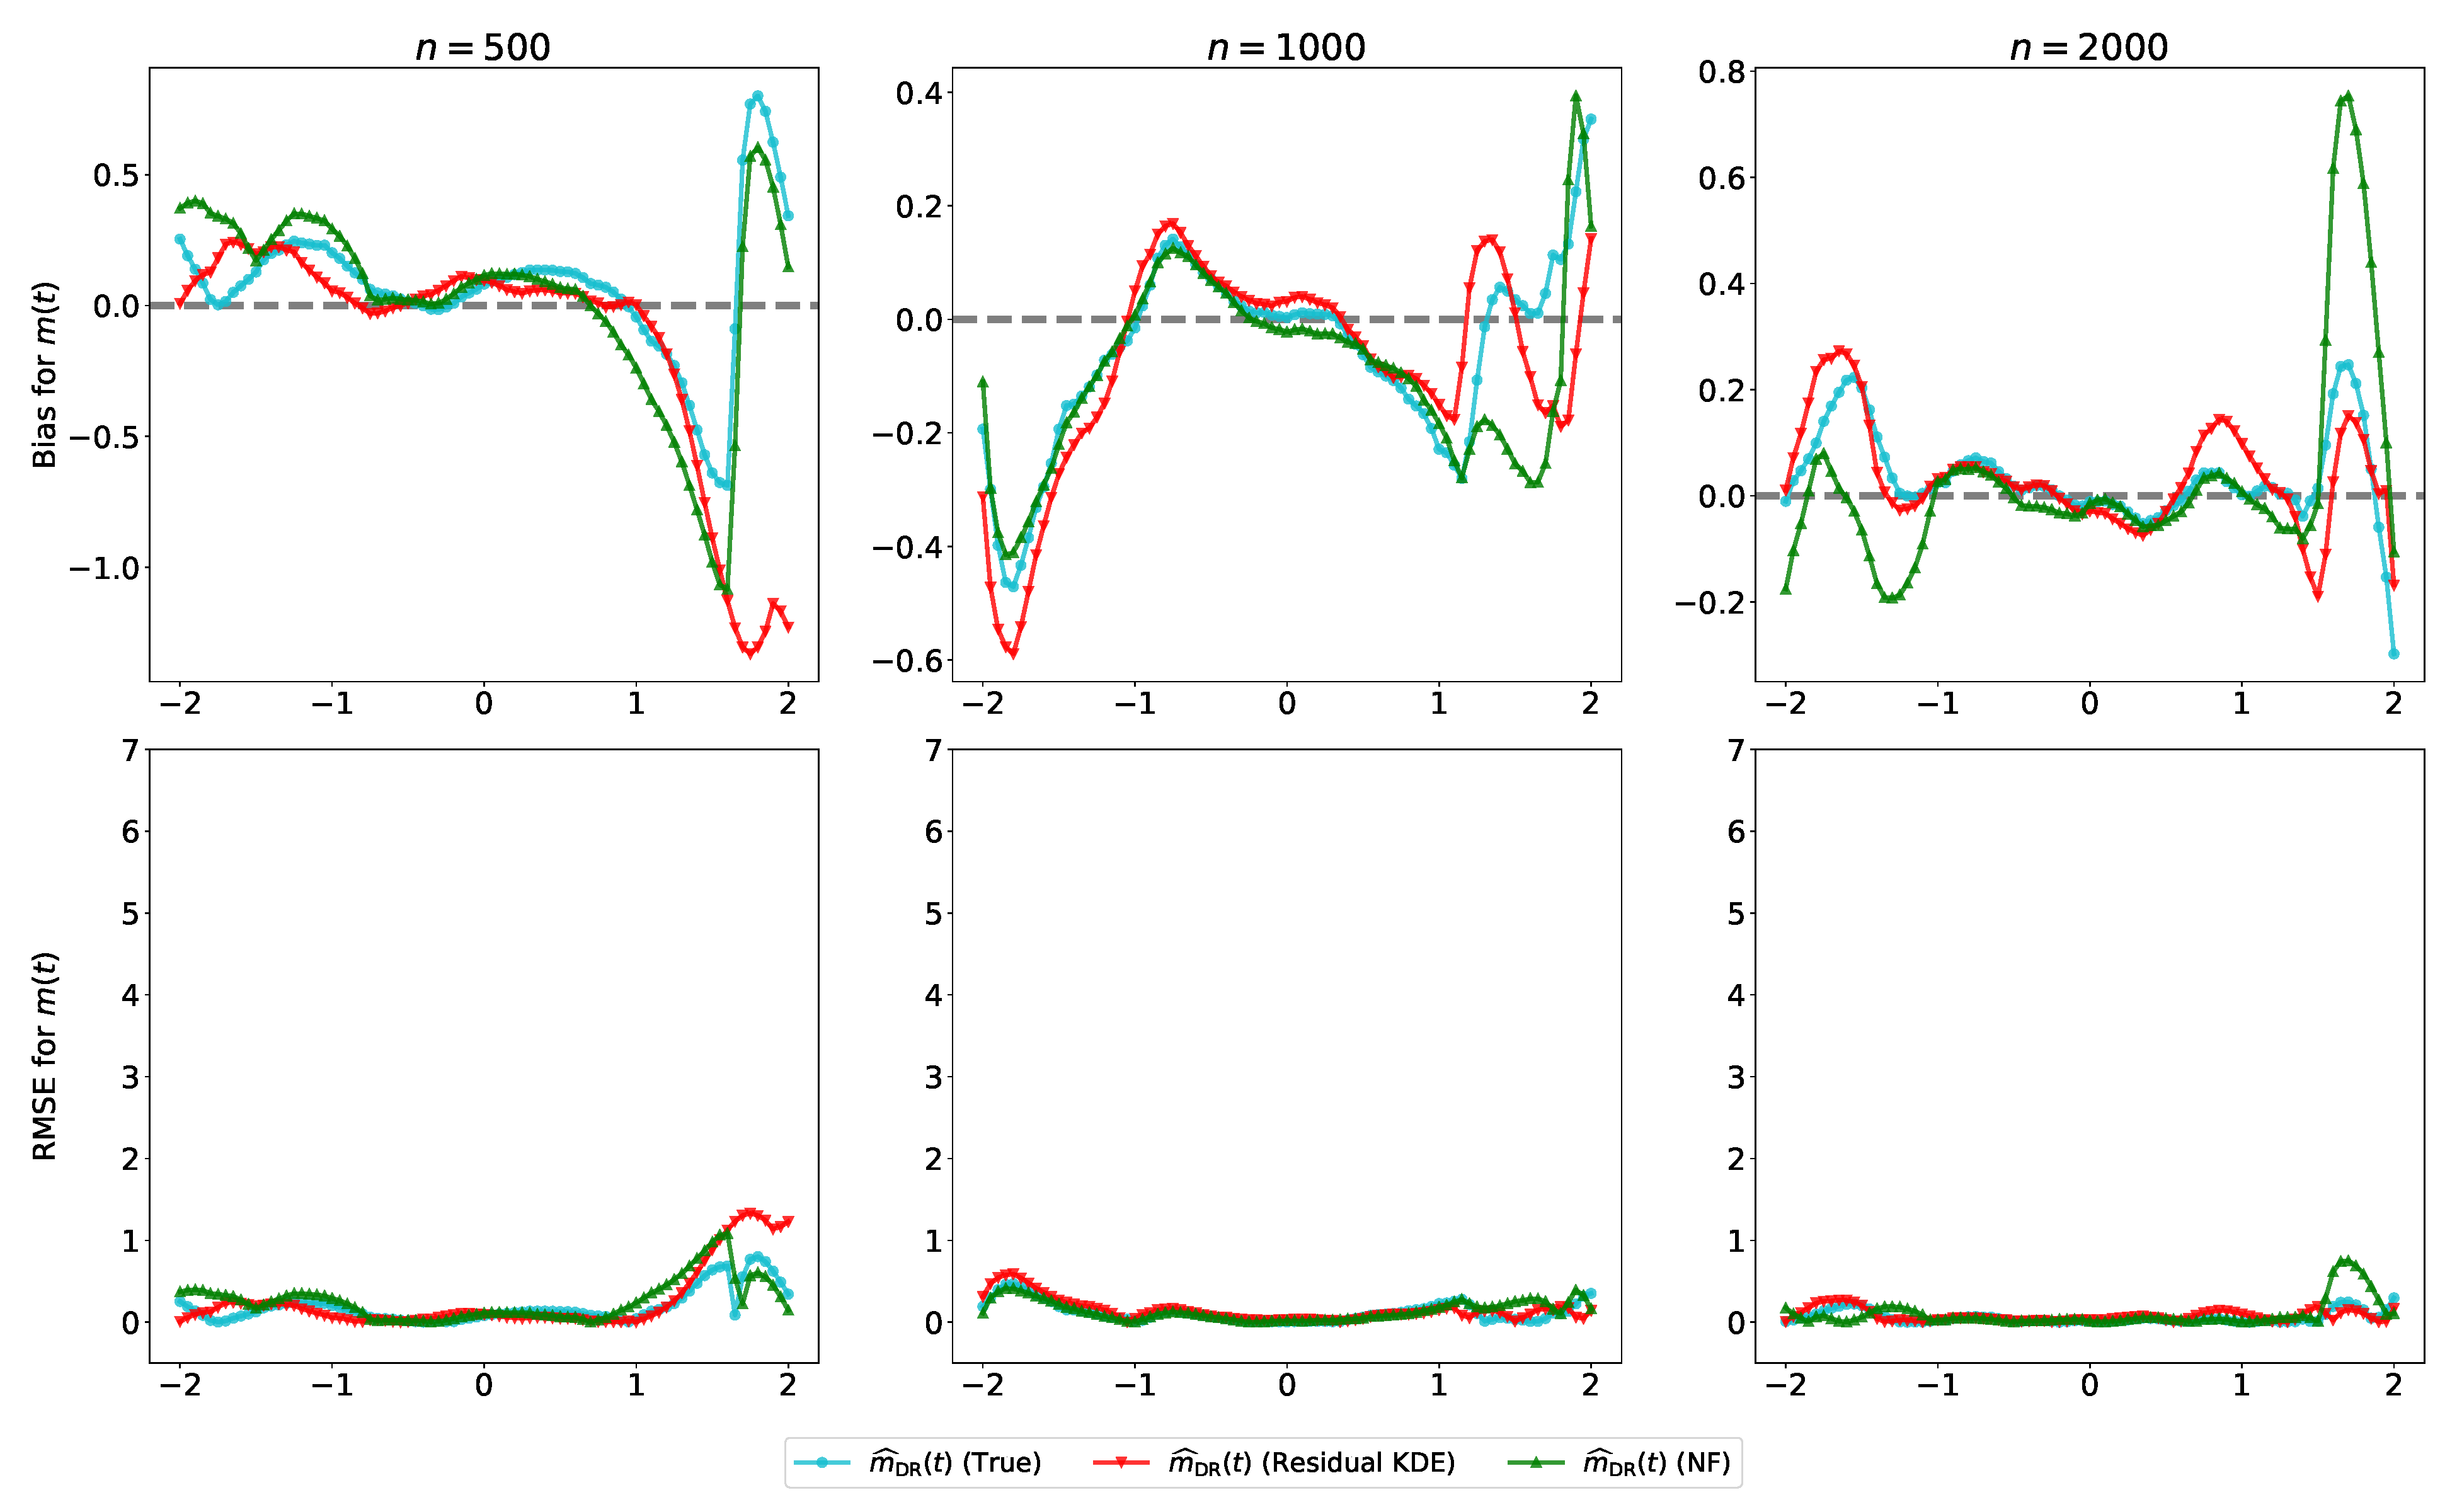
\includegraphics[width=0.95\linewidth]{../../figures/m.pdf}
    \caption{\scriptsize Bias and RMSE for dose--response $m(t)$ across sample sizes ($n = 500, 1000, 2000$)}
  \end{figure}

\end{frame}

%%% SLIDE 6: Conclusion %%%
\begin{frame}
  \frametitle{Conclusion \& Next Steps}

  \textbf{Summary:}
  \begin{itemize}
    \item NF provides accurate, tuning-free GPS estimation for continuous treatments
    \item NF-based AIPW estimator achieves comparable performance to oracle (true GPS)
    \item Avoids kernel/bandwidth sensitivity of KDE
  \end{itemize}

  \vspace{0.3cm}
  \textbf{Next steps:}
  \begin{itemize}
    \item Theoretical properties of NF-based GPS estimator
    \item Application to political science data with continuous treatment
    \item Comparison with other ML-based GPS estimators (e.g., random forest)
  \end{itemize}

\end{frame}

%%% SLIDE 7: References %%%
\begin{frame}%[allowframebreaks]
  \frametitle{References}

  \scriptsize


  \bibliographystyle{ecta}
  \bibliography{../ref}

\end{frame}

\end{document}
